\documentclass{article}
\usepackage{lipsum}
\usepackage{amsmath}
\usepackage{hyperref}
\usepackage{xcolor}
\usepackage{amsfonts}
\usepackage{graphicx}
\topmargin=-0.65in    % Make letterhead sftart about 1 inch from top of page
\textheight=9.10in    % text height can be bigger for a longer letter
\oddsidemargin=-0.1in % leftmargin is 1 inch
\textwidth=6.7in   % textwidth of 6.5in leaves 1 inch for right margin

% some shortcuts
\newcommand{\ea}{\textit{et al. }} 
\newcommand{\eg}{\textit{e.g. }} 
\newcommand{\ie}{\textit{i.e. }} 
\newcommand{\la}{\langle}
\newcommand{\ra}{\rangle}
\newcommand{\cg}{\color{gray}}
\newcommand{\fs}{\footnotesize}
\setlength{\parindent}{0mm}

%%%%%%%%%%%%%%%%%%%%%%%%%%%%%%%%%%%%%%%%%%%%%%%%%%%%%%%%%%%%%%%%%%%%%%%%
%%%%%%%%%%%%%%%%%%%%%%%%%%%%%%%%%%%%%%%%%%%%%%%%%%%%%%%%%%%%%%%%%%%%%%%%
%%%%%%%%%%%%%%%%%%%%%%%%%%%%%%%%%%%%%%%%%%%%%%%%%%%%%%%%%%%%%%%%%%%%%%%%
%%%%%%%%%%%%%%%%%%%%%%%%%%%%%%%%%%%%%%%%%%%%%%%%%%%%%%%%%%%%%%%%%%%%%%%%
\begin{document}

\author{Outline by: Evangelos Sariyanidi}

%%%%%%%%%%%%%%%%%%%%%%%%%%%%%%%%%%%%%%%%%%%%%%%%%%%%%%%%%%%%%%%%%%%%%%%%
%%%%%%%%%%%%%%%%%%%%%%%%%%%%%%% OUTLINE %%%%%%%%%%%%%%%%%%%%%%%%%%%%%%%%
%%%%%%%%%%%%%%%%%%%%%%%%%%%%%%%%%%%%%%%%%%%%%%%%%%%%%%%%%%%%%%%%%%%%%%%%
\title{\bf Outline of Foundations of Signal Processing}
\maketitle
\section*{Chapter 4 -- Functions and Continuous-time Systems}
Main discussion around Continuous-Time Fourier Transform (CTFT) and Fourier Series (FS), subjects like Laplace Transform and Cont. Stochastic Processes are touched very briefly.

Particularly useful is the usage of CTFT to determine the smoothness or differentiability of a function $x$.


\begin{itemize}
\item Smooth functions	{\cg Global \textit{smoothness} of a function described via its continuity and continuity of its derivs}
\item Systems: Continuous-Time (CT) systems {\cg are operators with functions as their input and output.} \\
{\cg\fs Linear, Memoryless, Causal, Shift-invariant, (BIBO) stable}
\item Differential equations {\cg can define most system types. They are typically solved via Fourier Laplace Transforms}
\item CTFT (or simply FT) is an operator $F:\mathcal{L}^2(\mathbb{R})\rightarrow \mathcal{L}^2(\mathbb{R})$
\begin{itemize}
\item Fourier Transform {\cg so popular because complex exponentials are eigenfunctions of LSI systems:}\\
{\cg $(h\ast v)(t) = \int\upsilon(t-\tau)h(\tau)d\tau=\int e^{j\omega(t-\tau)}h(\tau)d\tau=\int h(\tau)e^{j\omega\tau}d\tau e^{j\omega t}$, i.e. $e^{j\omega t}$ comes out as eigenfunction \\
{\fs
Defn, Fourier Transform(FT): $X(\omega) = \int\limits_{-\infty}^{\infty}x(t)e^{-j\omega t} dt$\\
Inverse FT (IFT): $x(t) = \frac{1}{2\pi}\int\limits_{\infty}^\infty X(\omega) e^{j\omega t}d\omega$}}
\item Fourier operator $F:\mathcal{L}^2(\mathbb{R})\rightarrow \mathcal{L}^2(\mathbb{R})$ is a unitary operator up to scaling factor $2\pi$! \\{\cg\fs (defn of unitary $U^{*}U=I$, alternatively $U$ is surjective AND $\la Ux,Uy \ra=\la x,y \ra$)\\
See more here: \url{https://people.math.osu.edu/gerlach.1/math/BVtypset/node32.html}}
\item Parseval equality, $||x||^{2}=\frac{1}{2\pi}||X||^2$ and $\la x,y \ra = \la X,Y \ra$ {\cg (equivalent with $F/\sqrt{2\pi}$ being unitary operator, see above)}
\item Properties of FT in Table 4.1 \#366.
\item Common transform pairs also in Table 4.1 (e.g. FT of box fn, Heaviside fn, Gaussian fn).
\item When the FT of a fn can't be evaluated directly, we can evaluate through IFT {\cg (e.g. FT of constant function, see Ex 4.6 \#365)}
\item !important! Differentation and Convolution via FT {\cg \--- see the relationship in Fig. \ref{fig:diff_conv}below}.
\item !IMPORTANT! FT facilitates the characterization of boundedness and continuousness (and differentiability)\\
{\cg\fs For some positive $\gamma, \epsilon$: \\
(i) $|X(\omega)| \le \frac{\gamma}{1+|\omega|^{1+\epsilon}} \implies $ $x$ is bounded and continuous (\ie $x \in C^{0}$) \\
(ii) $|X(\omega)| \le \frac{\gamma}{1+|\omega|^{1+\epsilon+q}} \implies $ $x\in C^{q}$ (has $q$ cont derivs) \\
(iii) $x \in C^{q}$ and $x$ is bounded (but not necess. cont.) $\implies$ $|X(\omega)| \le \frac{\gamma}{1+|\omega|^{1+q}}$  \\
(to understand these better see example 4.8 \#376)
}
\item Lipschitz Regularity {generalizes the above to differentiablity of fractional order:}\\
\item !critical! Lipschitz regularity can describe whether a fn is continuous ALMOST everywhere {\cg (\ie being of Lipschitz order of $1-\epsilon$ for any $\epsilon>0$  means being almost of order $1$, see \#378)}
{\cg\fs
Let $\alpha \in [0,1)$. Then $x$ is \textit{pointwise Lipschitz} of order $\alpha$ at $t_0$ when $|x(t)-x(t_0)|\le c|t-t_0|^\alpha$. \\
In FT context; a fn $x$ is bounded and \textit{uniformly} Lipschitz over $\alpha$ when: $\int\limits_{-\infty}^{\infty} |X(\omega)|(1+|\omega|^\alpha)d\omega < \infty$
}
\end{itemize}
\item Laplace Transform: Extends FT with more general complex exponentials. 
\item Fourier Series (FS) is an operator $F: \mathcal{L}^2(\mathbb{R}) \rightarrow \ell^2(\mathbb{Z})$\\
{\cg Defined for periodic signals over a single period $T$: \\
$X_k=\frac{1}{T}\int\limits_{-T/2}^{T/2}x(t)e^{-j(2\pi/T)k}dt$, $k \in \mathbb{Z}$. \\
Reconstruction via FS: $x(t) = \sum\limits_{k\in\mathbb{Z}}X_k e^{j(2\pi T)kt}, t\in [-\frac{T}{2},\frac{T}{2})$
}
\begin{itemize}
\item Properties at Table 4.3 (\#386)
\item FS is a \textbf{countable} orthonormal basis\\
{\cg The set $\{\phi_k\}_{k\in\mathbb{Z}}$ with $\phi_k(t)=\frac{1}{\sqrt{T}}e^{j(2\pi/T)kt}$ forms an orthonormal basis for $\mathcal{L}^{2}([-\frac{T}{2},\frac{T}{2}))$ \\
{\fs To prove this, show that i) $\la \phi_k,\phi_l \ra=\delta_{k-l}$ (see page \#384) and ii) any $x\in\mathcal{L}^{2}([-\frac{T}{2},\frac{T}{2}))$ is in $\overline{\text{span}}(\{\phi_k\}_{k\in\mathbb{Z}})$ (book not clear, see Supp1, Section 7.1)}
}
\item Thm 4.15 (\#384) Fundamental 3-fold Theorem:\\
{\cg\fs
Let $\hat{x}$ be the FS reconstruction of $x$ from $X=Fx$. Then:\\
i) $\mathcal{L}^2$ inversion: $||x-\hat{x}||=0$ \\
ii) (Parseval) $||x||^2=T\sum\limits_{k\in\mathbb{Z}}|X_k|^2$ and $\la x,y \ra = T\sum_{k\in\mathbb{Z}}X_kY^{*}_k$\\
iii) Least-squares approx: The fn $\hat{x}_N=X_k e^{j(2\pi/T)kt}$ is the \textit{least-squares approx} of $x$ on subspace $\overline{\text{span}}(\{\phi_k(t)\}^N_{k=-N})$

}
\item Defn \-- Dirac Comb: $s_T(t)=\sum\limits_{n\in\mathbb{Z}}\delta()  $
\item Relation bw FT and FS: $X(\omega) = 2\pi \sum\limits_{k \in \mathbb{Z}}X_k\delta (\omega-\frac{2\pi}{T}k)$
\item Furthermore: when the FT of {\cg $\tilde{x}=1_{[-T/2,T/2)}x$ exists, the FS of $x$ exists too.}
\item Thm 4.16 (\#392) Poisson Sum Formula (!critical! for sampling theorem): \\
{\cg Let $x$ be a fn with sufficient decay for the periodization $(s_T*x)(t)=\sum_{n\in\mathbb{Z}}x(t-nT)$ to converge absolutely for all $t$.\\
Then (simplified version): $\sum_{n\in\mathbb{Z}}x(n)=\sum_{k\in\mathbb{Z}}X(2\pi k)$ --- see \#392 }
\item Regularity and spectral decay --- {\cg like FT, FS can too be used to characterize the boundedness and continuity of fns:}
{\cg\fs For some positive $\gamma, \epsilon$: \\
(i) $|X_k| \le \frac{\gamma}{1+|k|^{1+\epsilon}} \implies $ $x$ is bounded and continuous (\ie $x \in C^{0}$) \\
(ii) $|X_k| \le \frac{\gamma}{1+|k|^{1+\epsilon}} \implies $ $x\in C^{q}$ (has $q$ cont derivatives) \\
(iii) $x \in C^{q}$ and $x$ is bounded (but not necess. cont.) $\implies$ $|X_k| \le \frac{\gamma}{1+|k|^{1+q}}$ 
}
\end{itemize}

\end{itemize}


\begin{figure}
\centering
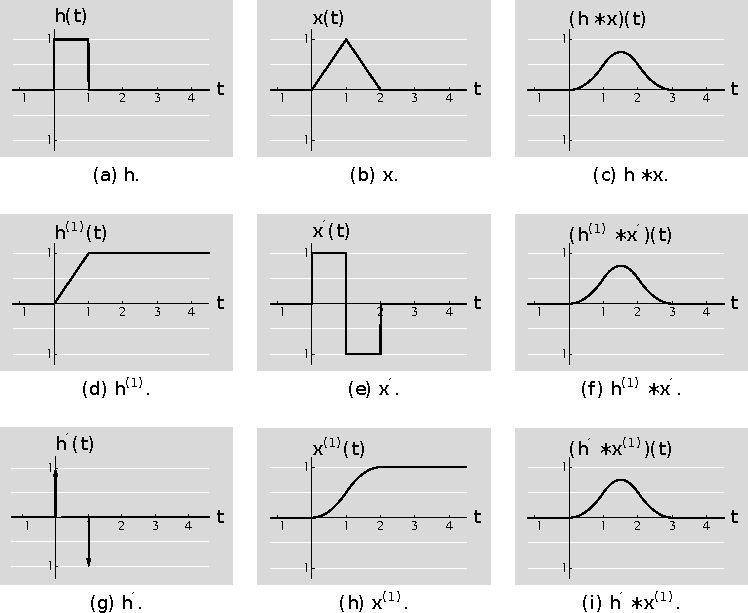
\includegraphics[scale=0.7]{fig/diff_conv.pdf}
\caption{The relation bw convolution and differentiation}
\label{fig:diff_conv}
\end{figure}


% https://www.youtube.com/watch?v=VXwXkME9uWU&list=PLMn2aW3wpAtOqo0g0OnHndXB1LnYBeMaX&index=1
\end{document}


